\chapter{Aryans Visit India}

\begin{longtable}{|>{\raggedleft}p{1.5cm}|p{8.5cm}|}
\multicolumn{2}{c}{\textbf{Table: 1}}\\ 
\hline
\textbf{Page \#} & \textbf{McGraw Hill Text} \tabularnewline
\hline
249 & Timeline: 1500 BCE: Aryans begin migrations to India \tabularnewline
\hline
249 & Timeline: 1000 BCE: Aryans control northern India \tabularnewline
\hline
248 & Aryan’s are shown bringing great changes to India \tabularnewline
\hline
253 & nomads settled in valleys along the Indus River in an area that is now Pakistan \tabularnewline
\hline
255 & ARYAN MIGRATIONS AND SETTLEMENTS \tabularnewline
\hline
255 & Meanwhile, groups of people called the Aryans (AR•ee•uhnz) migrated to India. Soon a new civilization emerged \tabularnewline
\hline
255 & Indo-European people lived in central Asia but began migrating to other places. Some moved west to Europe or south to Iran. The Aryans went to India. \tabularnewline
\hline
255 & Like most Indo-Europeans, the Aryans raised cattle for meat, milk, and butter. They moved from place to place to find pastures and water for their cattle. The Aryans were expert horse riders and hunters, as well as fierce warriors. As they moved about, the Aryans sometimes raided nearby villages for food. \tabularnewline
\hline
259 & 4. EXPLAINING How did the Aryans change their way of life after they settled in India? \tabularnewline
\hline
259 & 5. ARGUMENTATIVE WRITING What is the most important way the Aryans affected India? Write a brief essay that summarizes your ideas about their impact. \tabularnewline
\hline
257 & As the Aryans settled into India, royal and commercial towns arose along India’s Ganges River. \tabularnewline
\hline
282 & 2. SEQUENCING Create a time line to arrange the events in the order that they occurred. A. Arab mathematicians adopt Indian symbols for the numbers 1−9. B. The Aryans begin to migrate into the Indus Valley. C. Chandragupta founds the Mauryan dynasty. D. The Gupta dynasty begins. E. Indus culture flourishes. F. Siddhartha Gautama, the Buddha, is born. G. Ashoka brings the Mauryan Empire to its height of power \tabularnewline
\hline
283 & IDENTIFYING Where did the Indus Valley civilization begin? \tabularnewline
\hline
284 & EXPLAINING EFFECTS How did the creation of iron tools affect the Aryans’ lifestyle?  \tabularnewline
\hline
\vbox{\hbox{}\hbox{256}\hbox{\phantom{\rule{0pt}{4.6cm}}}} & 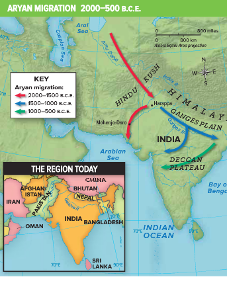
\includegraphics[scale=0.5]{figures/chap4-fig1.png} \tabularnewline
\hline
251 & \centering
\includegraphics[scale=0.5]{figures/chap4-fig2.png}\\ \raggedright ANALYZING KEY IDEAS AND DETAILS\\ Read closely to determine how the Aryans changed India. Use a diagram like this one to summarize your findings. \tabularnewline
\hline
255 & From about 1500 to 1000 B.C.E., bands of Aryans moved throughout India. These groups mixed with the descendants of the Indus Valley people. Together, they created a new culture. Over time, the Aryans in India adopted a new way of life. \tabularnewline
\hline
284 & SUMMARIZING What effect did the Aryans have on the Indus Valley civilization? \tabularnewline
\hline
254 & For example, the ruins show that cities’ royal palaces and temples may have been enclosed in a fortress. \tabularnewline
\hline
254 & 2. INFERRING What does the construction of fortresses around palaces and temples reveal about the Indus Valley culture? \tabularnewline
\hline
255 & THE INDO-EUROPEANS \tabularnewline
\hline
255 & The Aryans began to make iron tools to clear forests so they could farm the land. \tabularnewline
\hline
256 & The Aryans lived in tribes. \tabularnewline
\hline
256 & Like most nomadic people, the early Aryans had no written language. After they settled in villages, they developed a written language called Sanskrit (SAN•skriht). Sanskrit gave people a way to record sales, trade, and land ownership. Eventually, Aryan hymns, stories, poems, and prayers were also written in Sanskrit. Later, they were recorded and collected into sacred texts known as the Vedas (VAY•duhs). Examples of the Vedas remain today. \tabularnewline
\hline
256 & The Aryans migrated into India and spread throughout the subcontinent. 1. PATTERNS AND MOVEMENT From what general direction did the Aryan migration flow? 2. HUMAN-ENVIRONMENT INTERACTION What physical features did the Aryans settle along during their first migrations? Why did they settle there? \tabularnewline
\hline
257 & The Vedas were composed over a long period of time, from 1500 to 500 B.C.E. This period in Indian history is known as the Vedic period. According to many scholars, people speaking Indic languages entered South Asia during this period. The Indic languages are part of the larger Indo-European family of languages. They included the ancient language of Sanskrit, as well as ancestors of many of the languages spoken in South Asia today. \tabularnewline
\hline
257 & Over time, speakers of the Indic languages spread across northern India in scattered groups and encountered speakers of another ancient language group known as Dravidian. As they made contact with each other, speakers of the Indic and Dravidian languages would exchange their beliefs and traditions. Centuries of cultural exchanges between these two groups would result in a single “Vedic” culture in India. \tabularnewline
\hline
259 & 4. EXPLAINING How did the Aryans interact with the Indus Valley people? \tabularnewline
\hline
\vbox{\hbox{}\hbox{248}\hbox{\phantom{\rule{0pt}{3.2cm}}}} & \vbox{\kern2pt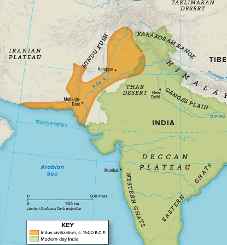
\includegraphics[scale=0.4]{figures/chap4-fig3.png}\kern2pt} \tabularnewline
\hline
IJ163 & ANALYZING EVENTS How did the Aryans influence the culture of India? Use the organizing web to show the various ways Aryans influenced India. \tabularnewline
\hline
IJ163 & The Impact of the Aryans on Indian Culture \tabularnewline
\hline
\end{longtable}


\section*{Analysis and Critique} 

These are in violation of California Education Codes 51501 and 60044—adverse reflection—and evaluation criteria clauses pertaining to historical inaccuracy, not including variety of perspectives and debates, perpetrating Eurocentric and Ethnocentric history, not remaining neutral in matters of religion (continuing with the missionary and imperialistic writings on Hinduism), and thereby instilling prejudice in Hindu and non-Hindu children against origins of Hinduism and Hinduism per se. 
\vskip 2pt

The present picture privileges the Aryan migration theory and is outdated in the light of current archaeological data and linguistic discourse. 
\vskip 2pt

The invasion or migrations of Aryans is a challenged theory with the archeologists having found NO ARCHAEOLOGICAL EVIDENCE WHATSOEVER to support either the earlier invasion of the Aryans of the Indian subcontinent or the migration of the Aryans to the Indian subcontinent. Further B.B. Lal (2005), an erstwhile Director General of the Archeological Survey of India, has argued that the dating of the coming of Aryans, as first suggested by Max Muller, was done on speculative basis, which Max Muller rescinded when challenged by his academic peers. Unfortunately, when an untruth gets recycled over a period, particularly at a time when there are no opposing voices to challenge because the history is being written by colonizing forces, it becomes the Truth. It is not for nothing that it is stated, “history is written by victors.” At first, the theory was that the Aryans invaded the Indian subcontinent around 1500 BCE. When no archeological support was found, a variant of the invasion theory—migration theory—was proposed. The date of the coming of the Aryans, however, did not change. Now if a theory gets shot down on the lack of evidence, a rational outcome is that one would drop the theory altogether. This did not happen and the invasion theory was replaced with the migration theory. Incidentally, there is no archeological support of the migration either. On the contrary, many Indian as well as western archeologists, such as Jim G. Shaffer and Diane A. Lichtenstein (2005), claim that the Indian civilization shows continuity without any break from much before 1500 BCE till the beginnings of the historical period. Shaffer and Lichtenstein write:

\begin{quote}
The modern archeological record for South Asia indicates a history of significant cultural continuity; an interpretation at variance with earlier eighteenth through twentieth-century scholarly views of South Asian cultural discontinuity and South Asian cultural dependence on western cultural influences.\footnote{J. G. Shaffer and Diane A. Litchenstein, “South-Asian Archeology and 	the Myth of Indo-Aryan Invasions,” in \textit{The 	Indo-Aryan Controversy: Evidence and Inference in Indian History}, eds.\ Edwin F. Bryant and Laurie L. Patton (New York: Routledge, 2005), 	93.}
\end{quote}

\noindent
The Aryan invasion—or migration—theory is based on the \textbf{racial superiority} of Europeans, outmoded eighteenth and nineteenth century paradigm, when it was accepted that people of European descent were superior to all other “races” of the world: if at all there was any civilization in any part of the world, it could only be the work of people with European ancestry. Shaffer and Lichtenstein are cognizant of the nexus between \textbf{racist presuppositions} and the Aryan invasion/migration theory and they write the following: 

\begin{quote}
The scholarly paradigm of the eighteenth and nineteenth centuries in conflating language, culture, race, and population movements has continued, with historical linguistic scholars still assiduously attempting to reconstruct a proto-Indo-European language, and attempting to link that language to a specific “homeland,” in order to define population migration away from the seminal geographic base. Suggestions for such a proto-Indo-European homeland range from Siberia to more recent efforts to tracing the homeland to Anatolia … and the Ukraine … and these efforts now incorporate human genetic studies … to verify the linguistic chronologies.\footnote{J. G. Shaffer and Diane A. Litchenstein, “South-Asian Archeology and 	the Myth of Indo-Aryan Invasions,” in \textit{The Indo-Aryan Controversy: Evidence and Inference in Indian History}, eds.\ Edwin F. Bryant and Laurie L. Patton (New York: Routledge, 2005), 93.}
\end{quote}

\noindent
However,

\begin{quote}
The current archeological and paleoanthropological data simply do not support these centuries old interpretative paradigms suggesting western, intrusive, cultural influence as responsible for the supposed major discontinuities in the South Asian cultural prehistoric record…. It is currently possible to discern cultural continuities linking specific prehistoric social entities in South Asia into one cultural tradition.\footnote{J. G. Shaffer and Diane A. Litchenstein, “South-Asian Archeology and the Myth of Indo-Aryan Invasions,” in \textit{The Indo-Aryan Controversy: Evidence and Inference in Indian History}, eds.\ Edwin F. Bryant and Laurie L. Patton (New York: Routledge, 2005), 93.}
\end{quote}

\noindent
Many aspects and cultural practices, including the city building plan, of the Harappans continued till the historic times as is evidenced in the excavation of a six hundred BCE city of Shishupalgarh by B. B. Lal (2011) and its incorporation in the \textit{Arthaśāstra} of Kautilya (1992), who was the mentor and teacher of Chandragupta Maurya. Lal (2009) has also shown how farming methods, plan of building houses, ornaments used by female populace including artifacts for wedding ceremonies, bedtime tales, lapidary methods, cooking methods including the use of pots and pans, games like chess, toys used by children, writing pad, etc. have continued to find their use in the current times in areas surrounding the Harappan civilization. In addition, figurines showing the traditional Hindu greeting Namaste, yogic poses later compiled in the Yoga sutras of Patanjali, fire alters used in Vedic ceremonies, seals depicting the Hindu Deity Shiva, iconic representation of Shiva in the form of \textit{Shivalinga} (in most Indian temples it is the iconic representation of Shiva that is used for worship even today) have been found in various sites of the Harappan culture. The above show the Vedic and indigenous roots of the Harappan culture rather than what the text argues for. 

Any life in current scholarship that the Aryan Invasion Theory (AIT) or its sibling the Aryan Migration Theory (AMT) today have is based on weak evidence of a group of Indo-European languages sharing similarities. It is weak evidence because one can very well argue that the migrations could have happened from India itself, which bestows upon the Indo-European language similarities. There is no dearth of scholars who have forcefully argued that the migration could have happened from India itself (see Talageri 2004, 2006, 2009; Elst 1993; Danino 2010; Kazanas 2015; Frawley 1993, 2001, 2016; and Feuerstein, Kak, and Frawley 2001). They have cited evidence, which supports the “migration out of India” thesis. In addition, there is also no textual evidence in any of the texts, held as Aryan texts such as the Vedas, Upanishads, Gītā, Rāmāyaṇa or Mahābhārata showing Aryans bringing changes impacting the social system or new beliefs with a basis that was outside of India.

In fact, in the beginning when William Jones made the announcement in late eighteenth century regarding the camaraderie of the Indo-European languages, India was held as the cradle of civilization and Sanskrit as the mother of all Indo-European languages. Using the evidence provided by Bryant (2002), Singh (in a forthcoming publication) has shown that the shift in the epicenter of the Aryan origins out of India and somewhere in Europe has been in direct proportion to Europe’s ascendency to colonial power. \textit{\textbf{The discourse of Aryan Invasion and migration is based in the racial superiority of European Aryans and we have already seen the havoc that it has caused before and during the Second World War. It is time that we completely drop this racist discourse, which explicitly manifests in the Aryan Invasion/ Migration theories.}} 

We would want to underline that antiquated imperialistic, colonial, racist, orientalist, and missionary writings that have been proven wrong on the basis of evidence essentially lead to adverse reflection on Hinduism and Indian heritage. 

There is another rub that must be taken into consideration. The Harappan civilization is considered a Bronze Age civilization. Now because it has been presumed that the Bronze Age civilization of the Harappans was ended by “invading or migrating Aryans,” the “Aryans” have been credited as bringing the Iron Age into India. With the continuity in prehistoric India the Harappan/Aryan is a fictitious divide. The Harappans, as they moved further eastwards, after the collapse of their predominantly urban civilization due to the drying of the river Sarasvati, they cleared new areas for habitation. We refer the readers to the colossal evidence for the above provided by archeologists like B. B. Lal, Jim Shaffer, Diane Litchenstein, Gregory Possehl, Jonathan Kenoyer, S. P. Gupta, and to writers like Michel Danino. 
\eject

Because McGraw Hill is pushing the migration theory through the back door, they did not realize that it was the “invasionists” who had suggested the fortress or the citadel around “palaces” and “temples.” The fact of the matter is that there are neither temples nor palaces in the Harappan culture. What you find are fire alters and in instances of Mohenjo-Daro and Dholavira, tanks which probably were used for ritualistic purposes (see Possehl 2002). 
%\vskip 1pt

The lack of palaces and temples reveal a social structure devoid of extreme hierarchy that were prevalent in contemporary ancient Egyptian and Mesopotamian cultures. If we take the contemporary mores into account, the civilization was far more advanced in terms of not creating socially oppressive hierarchies. This fact should neither be omitted nor altered, for its correct representation will be a big step in creating pride and confidence in the heritage of the Indian American children. 
%\vskip 1pt

Given there are no Aryans separate from Ancient Indians, there is no basis for the statement that Aryans lived in tribes. We would not see emergence of ancient cities like Varanasi if that were the case (which has been dated to 2000 BCE).\footnote{Jhimi Mukherjee Pandey, “Varanasi is as Old as Indus Valley 	Civilization, finds III-KGP Study” last modified Feb 26, 2016. 	\url{http://www.timesofindia.com/city/kolkata/Varanasi-is-as-old-as-Indus-valley-civilization-finds-IIT-KGP-study/articleshow/51146196.cms}} 
%\vskip 1pt

The text continues to go on teaching the antiquated Indo-European origin theory of the Aryans stating that these people brought in the Veda and Sanskrit. 
%\vskip 1pt

Sanskrit is a spoken and written language. It was not purely a “written language.” It has been written in many scripts over time (e.g., Brahmi and Devanagari). 
%\vskip 1pt

Further, the Vedas pre-date the written script of Sanskrit by centuries. It is a well-known fact that the Vedas were passed on orally for hundreds of years before they were written down. To say that writing was developed and followed by the creation of the Vedas is incorrect.
%\vskip 1pt

The Vedas were compiled in their present form before 1500 BCE. The Vedic dating of 1500--600 BC privileges the colonial theories of the origins of Sanskrit based on linguistics and the Aryan invasion/migration theories. Further as Lal (2005) has shown that the coming of Aryans, to begin with, was arbitrarily placed around 1500 BCE; consequently, the date of the Vedas was assigned arbitrarily too.

The Aryan / Dravidian divide is contingent upon the Aryan Invasion / Migration Theories and given that the theories themselves are wrong, all contentions in the book regarding the Aryans and the Dravidians become suspect and contentious. \textit{\textbf{Besides, the Aryan/Dravidian categorization is based on unscientific and outmoded race-based theories of the bygone eras}} (see Robb 1995; Trautmann 2005). 

In addition, the present text implies that Tamils were not Hindus, by placing them as separate from people from Northern India. Tamil sages and others from South India were Hindu and responsible for development of key aspects of Hinduism. In fact, multiple sub-cultures and languages from across India contributed to the development of Hinduism.

We have shown through colossal evidence that there is no trace of any invasion or migration of the “Aryans” coming into the Indian subcontinent and that the invasion or migration of the Aryans was based in racial superiority of Europeans and colonial, imperial, and orientalist writings on India and Hinduism. Given that the McGraw Hill narrative is that the Aryans came from outside the Indian subcontinent and founded Hinduism, it reflects significantly adversely on Hinduism and Hindus (basically suggesting that indigenous Hindus were not capable of having a religion of their own). It therefore indoctrinates students against Hinduism. We will not belabor this point but all contentions in the textbook connecting the invasion/migration of Aryans with origins of or discussion on Hinduism are adverse reflections on Hinduism and Indian heritage.

\begin{thebibliography}{99}
\bibitem{chap4-key1} Bryant, Edwin. \textit{The Quest for the Origins of the Vedic Culture: The Indo-Aryan Migration Debate}. New York: Oxford University Press, 2001.
\bibitem{chap4-key2} Danino, Michel. \textit{The Lost River: On the Trail of the Sarasvati}. New York: Penguin Books, 2010.
\bibitem{chap4-key3} Elst, Koenraad. \textit{Indigenous Indians: Agastya to Ambedkar}. New Delhi: Voice of India, 1993.
\bibitem{chap4-key4} Feuerstein, Georg, Subhash Kak, and David Frawley. \textit{In Search for the Cradle of Civilization}. Wheaton: Quest Books, 2001.
\bibitem{chap4-key5} Frawley, David. \textit{Gods, Sages, and Kings: Vedic Secrets of Ancient Civilization}. New Delhi: Motilal Banarasi Dass, 1993.
\bibitem{chap4-key6} Frawley, David. \textit{The Rig Veda: And the History of India}. New Delhi: Aditya Prakashan, 2001. 
\bibitem{chap4-key7} Frawley, David. \textit{The Myth of the Aryan Invasion of India}. Rev. ed. New Delhi: Voice of India, 2016.
\bibitem{chap4-key8} Kautilya. \textit{The Arthaśāstra}. Translated and edited by L. N. Rangarajan. New Delhi: Penguin Books, 1992.
\bibitem{chap4-key9} Kazanas, Nicholas. \textit{Vedic and Indo-European Studies}. New Delhi: Aditya Prakashan, 2015.
\bibitem{chap4-key10} Lal, B. B. \textit{How Deep are the Roots of Indian Civilization? Archaeology Answers}. New Delhi: Aryan Books International, 2009.
\bibitem{chap4-key11} Lal, B. B. “Aryan Invasion of India: Perpetuation of a Myth.” In \textit{The Indo-Aryan Controversy: Evidence and Inference in Indian History}, edited by Edwin F. Bryant and Laurie L. Patton, 50--74. New York: Routledge, 2005.
\bibitem{chap4-key12} Shaffer, J. G., and Diane A. Litchenstein. “South-Asian Archeology and the Myth of Indo-Aryan Invasions.” In \textit{The Indo-Aryan Controversy: Evidence and Inference in Indian History}, edited by Edwin F. Bryant and Laurie L. Patton, 75--104. New York: Routledge, 2005.
\bibitem{chap4-key13} Singh, Kundan. \textit{Sri Aurobindo’s Invalidation of the Aryan Invasion Theory and Contemporary Western Archeological Evidence}. Springer, forthcoming. 
\bibitem{chap4-key14} Talageri, Shrikant. \textit{The Rigveda: A Historical Analysis}. Rev.\ ed.\ New Delhi: Aditya Prakashan, 2004. 
\bibitem{chap4-key15} Talageri, Shrikant. \textit{The Aryan Invasion Theory: A Re-appraisal}. Rev.\ ed.\ New Delhi: Aditya Prakashan, 2006.
\bibitem{chap4-key16} Talageri, Shrikant. \textit{The Rigveda and the Avesta: The Final} Evidence. New Delhi: Aditya Prakashan, 2009.
\bibitem{chap4-key17} Possehl, Gregory L. \textit{The Indus Civilization}. Walnut Creek, CA: Alta Mira Press, 2002
\bibitem{chap4-key18} Robb, Peter, ed.\ \textit{The Concept of Race in South Asia}. New Delhi: Oxford University Press, 1995. 
\bibitem{chap4-key19} Trautmann, Thomas R. \textit{The Aryan Debate}. New Delhi: Oxford University Press, 2005.
\end{thebibliography}
\newpage

\begin{longtable}{|>{\raggedleft}p{1.5cm}|p{8.5cm}|}
\multicolumn{2}{c}{\textbf{Table: 2}}\\ 
\hline
\textbf{Page \#} & \textbf{McGraw Hill Text} \tabularnewline
\hline
257 & Texts in the Dravidian languages also began to appear around 300 B.C.E. From this time until the end of the 1st century C.E. there was a large number of written works produced in Dravidian languages. \tabularnewline
\hline
\end{longtable}

\section*{Analysis and Critique} 

This is in violation of California Education Codes 51501 and 60044—adverse reflection—and evaluation criteria clauses pertaining to historical inaccuracy, not including variety of perspectives and debates, perpetrating Eurocentric and Ethnocentric history, not remaining neutral in matters of religion (continuing with the missionary and imperialistic writings on Hinduism), and thereby instilling prejudice in Hindu and non-Hindu children against origins of Hinduism and Hinduism per se. 

The discussion of “Dravidian languages” is derived from the racist orientalist discussion on Hinduism, coming from the Aryan/Dravidian divide and is in effect indoctrinating students against Hinduism when it would have been more appropriate to speak of “early form of literary Tamil.” 
